
\section{Playing a Card}
\label{Section_PlayingACard}
\begin{figure}[ht]
	\begin{minipage}[t][6cm][t]{0.5\textwidth}
		\textbf{Play} - You may play up to two cards per turn. \\
		\textbf{Pay} - Cards either have no cost or an element cost. To pay  a element cost, remove the stated amount of element markers from the corresponding field on the wheel back into the stash.
		Most often, the element cost is optional. If the cost is not optional, you may not play it without paying the element cost.
		
		\begin{tcolorbox}[colframe=black, colback=white]
			When playing a card, you execute all effects from top to bottom, going line by line. All effects \textbf{must} to be used if possible. Different lines can target different targets.
		\end{tcolorbox}
		
	\end{minipage}	
	\begin{minipage}[t][6cm][t]{0.5\textwidth}
		\centering
		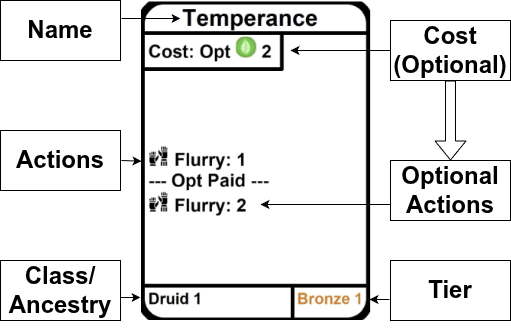
\includegraphics[width=0.9\linewidth, valign=t]{ExplanationPics/ActionCard.drawio.png}
	\end{minipage}
\end{figure}


\begin{figure}[ht]
	\label{fig_SingleTarget}
	\begin{minipage}[t][6cm][t]{0.5\textwidth}
		\centering
		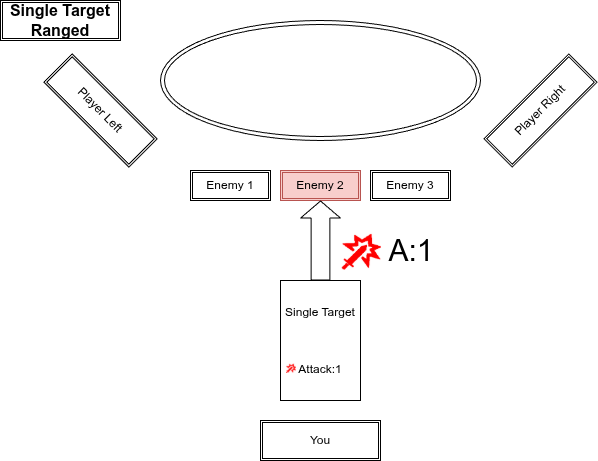
\includegraphics[width=0.9\linewidth, valign=t]{ExplanationPics/TargetingSingle.drawio.png}
	\end{minipage}	
	\begin{minipage}[t][6cm][t]{0.5\textwidth}		
		\textbf{Actions} - The most common actions are \symAttack attacks, boons and banes and  element generation.
		
		\textbf{Targeting} - By default, one action targets any one of your enemies (\textit{See left}).
		If multiple actions are listed in a single line, all of them must affect the same target.
		If multiple actions are listed in separate lines, they may affect different targets.
		Beneficial actions such as healing , shield etc. target yourself by default. \\
		\textbf{Ranged} - If the card has the keyword "Ranged" all actions may target any enemy (or in case of boons a player) to your left and right or in front of you. (\textit{See below})
	\end{minipage}
\end{figure}



\begin{figure}[ht]
	\label{fig_RangedSingleMultiTarget}
	\begin{minipage}[t][6cm][t]{1\textwidth}
		\centering
		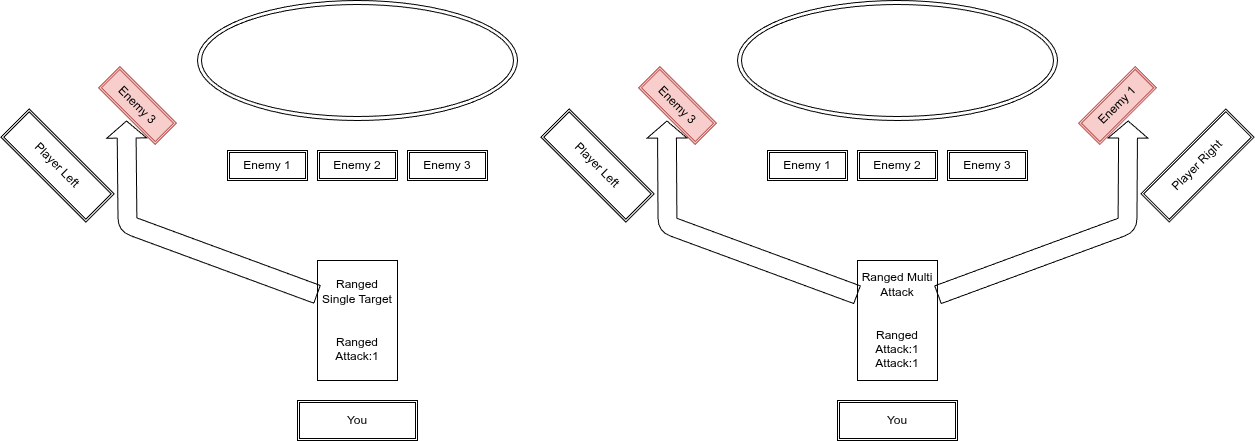
\includegraphics[width=0.9\linewidth, valign=t]{ExplanationPics/TargetingRanged.drawio.png}
	\end{minipage}	
\end{figure}

\begin{tcolorbox}[colframe=black, colback=white]
	If you have multiple attacks (or other effects) across multiple lines, you may choose new targets when you make each attack.
\end{tcolorbox}

\newpage

\textbf{AOE} - Some cards have an Area Of Effect.
AOE cards may target enemies that are adjacent to one another (\textit{See below}), in the pattern shown on the picture. Enemies of different players are never count as adjacent to each other, and AOEs may not flow over to another player zone.
All attacks and banes on the card are applied to each enemy targeted by the AOE.

\begin{figure}[ht]
	\label{fig_AOE}
	\begin{minipage}[t][13cm][t]{1\textwidth}
		\centering
		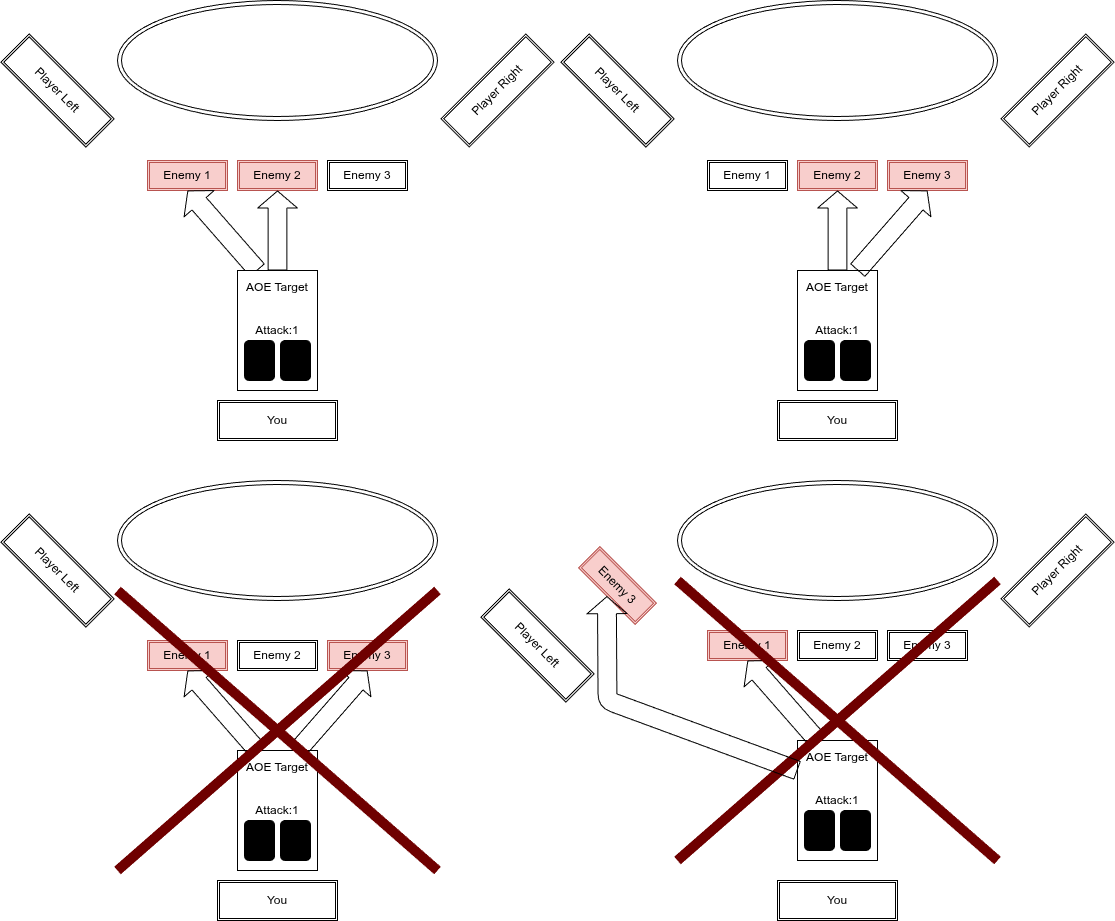
\includegraphics[width=0.9\linewidth, valign=t]{ExplanationPics/TargetingAOE.drawio.png}
	\end{minipage}	
\end{figure}

\textbf{Attack \symAttack} - To perform an attack, first select an enemy to attack.
Then, draw a modifier from you modifier deck, and add its value to the attack.
Every Deck also has a *2 and a *0. In that case, multiply your attack value by two (or  zero) after everything else was applied.
Modifiers are drawn and applied separately for each enemy attacked. This applies to multiple lines of attacks, as well as AOE attacks.

\textbf{Elements \symFire \symEarth \symMetal \symWater \symWood} - To generate elements, check how many element symbols are pictured on the card, and move that many markers from the stash to the wheel, on the corresponding field.

\textbf{Opt cost} - Cards with optional costs have a line with the word OPT going through the card with additional actions below the line.
If the optional cost was paid, the actions below the line must be used. If the cost was not paid, they cannot be used.

\textbf{Blaze \symBlaze} - Cards with blaze also have a line, but with the text Blaze:X instead of OPT.
If you play one of these cards as the first card on your turn, you must discard X cards, and use the actions below the line.
When played as the second card in a turn, the blaze action does nothing -- no cards are discarded, and the actions below the line are ignored.

\textbf{Boons \& Banes} - To apply a boon or bane, choose a target, then put the listed number of boons or banes on the target. \textit{See also page \pageref{Section_BoonsBanes}}

\textbf{Healing \symHeal} - Healing restores life by the stated amount. 

\textbf{Discard} - After playing a card, put it into your discard pile.
\begin{tcolorbox}[colframe=black, colback=white]
	If there are no enemies in front of you all your cards have ranged
\end{tcolorbox}
\newpage

\subsection*{Ancestry Dice}

The Ancestry Dice acts as an a source of random chance. Fighting is a risky business, and sometimes an attack may take an unexpected turn.
You usually start with two Ancestry dice.
Over the course of the game, you add more Ancestry Dice.
\begin{tcolorbox}[colframe=black, colback=white]
	%If you have played table top RPGs before, you may know the concept from rolling a 20 sided dice to determine the outcome of an action.
	Hier könnte ihre Werbung stehen.
\end{tcolorbox}

\textbf{Modify all  attacks \symAttack} - All  attacks (and only attacks) are modified by default. Modification usually changes how much damage your attack does. 
To determine the final damage, roll all Ancestry dice from your Dice Pool and add its combined value to the attack.

\textbf{Advantage \symAdvantage} - Advantage gives you an additional chance to hit good modifiers.
%todo which type of advantage do we use
After having rolled your dice before modifing the attack you can use one Advantage to reroll a dice. You may repeat this by using additional advantages

\textbf{Passive Interaction} - Some class passives allow you to modify healing or poison.
If you have one of those classes, modify your poison and heal actions  as you would modify an attack.

\fbox{\parbox[4cm]{\textwidth}{Picture: Children: Half elf, thyger and silverkin playing a dice game.}}

\begin{tcolorbox}[colframe=black, colback=white]
	After every player has finished playing their cards, move to the enemies turn. Indicate this by turning your leftmost enemy by 90 degrees. Coordination is important here, speak with the group to ensure that no one is still playing out their turn.
\end{tcolorbox}
